\section{Prototipo realizacija}

Šis skyrius aprašo praktinę rašto darbo pusę -- debesų kompiuterijos technologijomis grįstos saityno peržiūros roboto realizacijos sprendimus. Architektūra ir naudojami įrankiai parinkti pagal 4 skyriuje apibrėžtus sistemos reikalavimus.

\subsection{Sistemos panaudojamumas}

Įgyvendinant prototipo architektūrą pagal 4 skyriuje išsikeltus reikalavimus, apibrėžtos pagrindinės veiklos, kurios sudaro sistemos funkcionalumą, jos matomos \ref{fig:use_case_diagram} paveikslėlyje pavaizduotoje UML panaudojamumo diagramoje.

\begin{figure}[htp!]
\centering
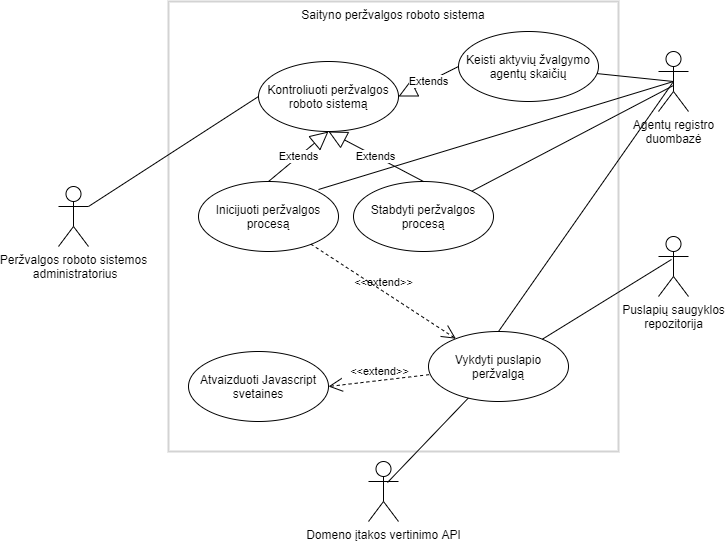
\includegraphics[scale=0.6]{img/Use_case_diagram.png}
\caption{UML žvalgymo roboto sistemos prototipo panaudojamumo diagrama}
\label{fig:use_case_diagram}
\end{figure}

Svarbu paminėti keletą aiškinamųjų aspektų apie \ref{fig:use_case_diagram} diagramoje pavaizduotas veiklas ir aktorius.


\textbf{Peržiūros roboto administratorius} -- klientinė programa, kontroliuojanti žvalgymo procesą. Klientas gali būti įvairių formų: komandinės eilutės programa, žiniatinklio, darbalaukio programa. Prototipo realizacijoje klientinė programa imituojama naudojantis \textit{„Service Bus Explorer“\footnote{https://github.com/paolosalvatori/ServiceBusExplorer}} įrankiu ir rankiniu būdu siunčiant žinutes į sistemos žvalgymo kontroliavimo eilę.

\textbf{Domeno įtakos vertinimo API} -- išorinis tarnybos serveris, kuris sugeba skalėje nuo 1 iki 100 įvertinti konkretaus domeno autoritetą, kuris reikalingas žvalgymo prioritizavimui. Prototipo įgyvendinimo metu naudota \textit{openrank.io\footnote{https://openrank.io/}} API paslauga, suteikianti 10000 nemokamų užklausų per 24 valandas. Akcentuotina, kad ši išorinė sistema nėra privaloma -- darbe pasirinkta etiško žvalgymo politika atsižvelgia į šią metriką siekiant nustatyti populiaresnes svetaines, kurias galima žvalgyti greičiau.

\textbf{Atvaizduoti Javascript svetaines} -- šis panaudojamumo atvejis yra vykdomas kaip atskira veikla po peržvalgos proceso, jei konkretus puslapis pasižymi dinaminės svetainės, kuri turinį generuoja klientinėje pusėje, savybėmis.

\subsubsection{Panaudojamumo atvejų paaiškinimai}
\ref{tab:use_case_table} lentelėje pateikti \ref{fig:use_case_diagram} diagramoje pavaizduotų panaudojamumo atvejų identifikatoriai ir detalesnis paaiškinimas:

% Table generated by Excel2LaTeX from sheet 'crawling_vs_scraping'
\begin{table}[ht]
  \centering
  \caption{Panaudojamumo atvejų paaiškinimai}
    \begin{tabular}{|p{2em}|p{13em}|p{20em}|}
    \hline
    \textbf{Id} & \textbf{Pavadinimas} & \textbf{Aprašymas} \bigstrut\\
    \hline
    U1.1 & Inicijuoti peržiūros procesą & Perkelti pradinį peržiūros URL adresų sąrašą į peržiūros eilę prieš tai patikrinti, ar URL adresai dar neperžiūrėti, ir sukurti pirmąjį peržiūros agentą, jam priskirti domeno vardo zoną \\
    \hline
    U1.2 & Stabdyti peržiūros procesą & Panaikinti visus aktyvius peržiūros robotus ir jų peržiūros eiles  \\
    \hline
    U1.3 & Keisti aktyvių peržiūros agentų skaičių & Padidinti arba pamažinti maksimalų leistiną peržiūros ir Javascript atvaizdavimo agentų kiekį sistemoje \\
    \hline
    U2 & Rekursyviai vykdyti puslapio peržiūrą & Aplankyti URL adresu nurodytą svetainę, išnagrinėti jos HTML turinį ir išgauti visas nuorodas, patikrinti, ar jos dar neperžiūrėtos, perduoti jas atitinkam peržiūros robotui  \\
    \hline
    U2.1 & Įvertinti, ar puslapis vykdo klientinį Javascript atvaizdavimą & Nustatyti, ar HTML dokumentas naudoja Javascript bibliotekas, kurios naudojamos klientinio atvaizdavimo vieno puslapio žiniatinklio programose, jei taip -- nusiųsti tokį URL adresą į Javascript atvaizdavimo eilę  \\
    \hline
    U2.2 & Įvertinti etiškos puslapio peržiūros laiko intervalą & Atsižvelgti į HTTP užklausos serverio atsakymo laiką, domeno populiarumą, robots.txt nurodytą leistiną peržiūros intervalą \\
    \hline
    U2.3 & Atvaizduoti Javascript svetaines & Naudojant Javascript variklį atvaizduoti pilną HTML turinį svetainėms, kurios naudoja klientinio atvaizdavimo bibliotekas \\
    \hline
    \end{tabular}%
  \label{tab:use_case_table}%
\end{table}%

\subsubsection{Atsekamumo matrica}

\ref{tab:requirements_use_case_traceability_matrix} lentelėje pateikta funkcinių, nefunkcinių reikalavimų ir nurodytų panaudojamumo atvejų atsekamumo matrica siekiant nurodyti, jog visi apibrėžti reikalavimai yra padengiami įgyvendinant peržiūros roboto prototipą.

% Table generated by Excel2LaTeX from sheet 'Sheet1'
\begin{table}[ht]
  \centering
  \caption{Reikalavimų ir panaudojamumo atvejų atsekamumo matrica}
    \begin{tabular}{|l|r|r|r|r|r|r|r|}
    \hline
          & \multicolumn{1}{l|}{\textbf{U1.1}} & \multicolumn{1}{l|}{\textbf{U1.2}} & \multicolumn{1}{l|}{\textbf{U1.3}} & \multicolumn{1}{l|}{\textbf{U2}} & \multicolumn{1}{l|}{\textbf{U2.1}} & \multicolumn{1}{l|}{\textbf{U2.2}} & \multicolumn{1}{l|}{\textbf{U2.3}} \bigstrut\\
    \hline
    \textbf{FR1} & \multicolumn{1}{l|}{\textbf{X}} &       &       &       &       &       &  \bigstrut\\
    \hline
    \textbf{FR2} &       &       &       & \multicolumn{1}{l|}{\textbf{X}} &       &       &  \bigstrut\\
    \hline
    \textbf{FR3} &       &       &       & \multicolumn{1}{l|}{\textbf{X}} &       &       &  \bigstrut\\
    \hline
    \textbf{FR4} & \multicolumn{1}{l|}{\textbf{X}} &       &       & \multicolumn{1}{l|}{\textbf{X}} &       &       &  \bigstrut\\
    \hline
    \textbf{FR5} &       &       &       & \multicolumn{1}{l|}{\textbf{X}} &       &       &  \bigstrut\\
    \hline
    \textbf{FR6} &       &       &       & \multicolumn{1}{l|}{\textbf{X}} &       & \multicolumn{1}{l|}{\textbf{X}} &  \bigstrut\\
    \hline
    \textbf{FR7} &       &       &       & \multicolumn{1}{l|}{\textbf{X}} &       &       & \multicolumn{1}{l|}{\textbf{X}} \bigstrut\\
    \hline
    \textbf{FR8} &       &       &       & \multicolumn{1}{l|}{\textbf{X}} &       &       & \multicolumn{1}{l|}{\textbf{X}} \bigstrut\\
    \hline
    \textbf{FR9} &       &       &       &       &       & \multicolumn{1}{l|}{\textbf{X}} &  \bigstrut\\
    \hline
    \textbf{FR10} &       &       & \multicolumn{1}{l|}{\textbf{X}} &       &       &       &  \bigstrut\\
    \hline
    \textbf{FR11} &       &       &       &       & \multicolumn{1}{l|}{\textbf{X}} &       & \multicolumn{1}{l|}{\textbf{X}} \bigstrut\\
    \hline
    \textbf{FR12} & \multicolumn{1}{l|}{\textbf{X}} &       &       & \multicolumn{1}{l|}{\textbf{X}} &       &       & \multicolumn{1}{l|}{\textbf{X}} \bigstrut\\
    \hline
    \textbf{NFR1} & \multicolumn{1}{l|}{\textbf{X}} & \multicolumn{1}{l|}{\textbf{X}} & \multicolumn{1}{l|}{\textbf{X}} & \multicolumn{1}{l|}{\textbf{X}} & \multicolumn{1}{l|}{\textbf{X}} & \multicolumn{1}{l|}{\textbf{X}} & \multicolumn{1}{l|}{\textbf{X}} \bigstrut\\
    \hline
    \textbf{NFR2} &       &       & \multicolumn{1}{l|}{\textbf{X}} &       &       &       &  \bigstrut\\
    \hline
    \textbf{NFR3} &       &       &       &       &       &       &  \bigstrut\\
    \hline
    \end{tabular}%
  \label{tab:requirements_use_case_traceability_matrix}%
\end{table}%


\subsection{Naudojama architektūra}

Prototipas rengiamas plačiai remiantis Kalifornijos Mersedo universiteto mokslininkų literatūrine medžiaga apie debesų kompiuterijos išskirstyto saityno žvalgymo roboto sistemą ir jos architektūrą, dizaino principus \cite{MercedCloudBasedWebCrawler}. Atsižvelgiant į darbo rašymo metus ir patobulėjusias debesų kompiuterijos tiekėjų siūlomas technologijas, pasiūlyta architektūra realizuojama pritaikius specifinius pokyčius pakeičiant realizacijos įrankius ir platformas. Šiame poskyryje aprašomi pasiūlytos architektūros pagrindiniai komponentai, pavaizduoti \ref{fig:mersed_architecture} diagramoje ir jų funkcinės atsakomybės.

\pagebreak

\begin{figure}[ht]
\centering
\includegraphics[scale=0.6]{img/Mersed_architektūra.png}
\caption{Mersedo universiteto mokslininkų pasiūlyta saityno peržiūros roboto architektūra \cite{MercedCloudBasedWebCrawler}}
\label{fig:mersed_architecture}
\end{figure}


\subsubsection{Centrinis žvalgymo variklis}
 
 Tai pagrindinis sistemos struktūrinis komponentas, kuris inicijuoja visą žvalgymo procesą ir kuria/naikina žvalgymo agentus. Pagrindiniai šio komponento veikimo etapai:
 \begin{enumerate}
     \item Inicializacija
     \begin{enumerate}
         \item Paimami pradiniai URL adresai iš žvalgymo adresų sąrašo
         \item Adresai sudedami į „Azure“ eilę prieš tai patikrinant, ar kiekvienas URL adresas dar nebuvo žvalgytas ( naudojamas \textit{„Azure NoSQL Table Storage“})
         \item Sukuriamas pirmasis žvalgymo agentas, jam priskiriama jo žvalgymo zona (svetainės serverio vardas)
     \end{enumerate}
     \item Ciklinis žvalgymo procesas
     \begin{enumerate}
         \item Iš žvalgymo eilės paimamas URL adresas
         \item Patikrinama, ar esamam URL adresui egzistuoja aktyvus agentas (SQL Agentų registro duombazė)
         \item Jei agentas egzistuoja, URL adresas ignoruojamas, nes priskirtas agentas jį apdoros
         \item Jei aktyvaus agento nėra, paskaičiavus aktyvių agentų skaičių A\textsubscript{aktyvūs} tikrinamas maksimalus leistinas agentų skaičius A\textsubscript{max} > A\textsubscript{aktyvūs}, jei sąlyga patenkinta, bandoma sukurti naują agentą ir jam priskirti URL adreso vardo zoną. Kitu atveju laukiama, kol sąlyga bus patenkinta (agentai baigs savo darbą).
         \item Kartojama nuo pirmo žingsnio
     \end{enumerate}
 \end{enumerate}
 
 \subsubsection{Žvalgymo agentas}

Šis komponentas iš žvalgymo eilės ima URL adresą, jei adreso vardo sritis sutampa su agentui priskirtu aptarnavimo vardo adresu, jis inicijuoja HTTP užklausą į nurodytą žiniatinklio serverį, parsiunčia HTML turinį, išgauna visas jame esančias nuorodas, kiekvienai jų patikrina, ar nuoroda dar neregistruota indeksų repozitorijoje ir atitinkamai perduoda aktyviam žvalgymo agentui, kurio zona sutampa su URL adreso vardo zona \cite{MercedCloudBasedWebCrawler}. Agentai užtikrina išskirstytos sistemos veikimo principą, juos galima dinamiškai pridėti, šalinti. Apibrėžtoje architektūroje nėra centrinio komunikacijos komponento, kuris deleguotų žvalgymo darbus agentams.

 \subsubsection{Agentų registras}
 
 Tai SQL duombazė, kurioje registruojami visi aktyvūs agentai, taip pat jie periodiškai išregistruojami aptikus, jog agentas kurį laiką nebuvo aktyvus. Šis komponentas yra bendras, todėl rašto darbo paskutiniame skyriuje, atliekant tyrimą, bus analizuojama, ar jis negali lemti „butelio kaklelio“ efekto.
 
 \subsubsection{„Azure“ žvalgymo eilė}
 
 Tai komponentas, kuris saityno žvalgymo sistemų literatūroje minimas kaip „žvalgymo pasienio“ (angl. -- \textit{Crawling Frontier}) komponentas, kuriame laikinai kaupiami žvalgytinų puslapių URL adresai \cite{EffectiveWebCrawling}. Žvalgymo agentai ir Centrinis žvalgymo variklis klausosi šios eilės žinučių ir jas apdoroja. Tai dar vienas bendrinis sistemos komponentas, todėl eksperimento metu taip pat bus stebimas jo veikimo pralaidumas. \cite{MercedCloudBasedWebCrawler} moksliniame darbe jau buvo atliktas šio komponento tyrimas ir įsitikinta, kad didinant žinučių kiekio apkrovą, komponento pralaidumas išlieka gana patovus. Naudota „Azure Storage Queues“ eilių paslauga. Šio rašto darbo tyrime naudojama „Azure Service Bus“ eilių infrastruktūra, todėl taip pat pakartotinai bus stebimas komponento veikimo pralaidumas.
 
 \subsubsection{„Azure“ NoSQL indeksų repozitorija}

Tai NoSQL rakto-reikšmės (angl. -- \textit{Key-Value}) tipo saugykla, kurioje agentai registruoja identifikuotus svetainių URL adresus, taip pat keičia tų adresų žvalgymo statusą, aptiktų URL nuorodų paminėjimų skaičių (angl. -- \textit{hit count}) \cite{MercedCloudBasedWebCrawler}.

\subsubsection{„Azure“ didelių objektų saugykla}

Šis komponentas aprašytoje architektūroje atsakingas už didelių multimedijos failų saugojimą -- nuotraukų, vaizdo įrašų, PDF dokumentų ir kitų žiniatinklio resursų, kurie nėra HTML dokumentai \cite{MercedCloudBasedWebCrawler}. Pasižymi tuo, jog gali talpinti didelius kiekius duomenų.

\subsubsection{Svetainės turinio analizatorius ir dublikatų aptikimas}

Vienas iš minimų sistemos komponentų -- svetainės turinio analizatorius -- semantiškai apdoroja nuskaitytą HTML dokumento turinį siekdamas nustatyti puslapio tematiką, pagrindinius raktinius žodžius, taip pat identifikuoti pasikartojančio, dublikuoto turinio svetaines. Šio prototipo įgyvendinimo ribose nebuvo numatytas semantinis svetainės turinio analizavimas, todėl plačiau šie komponentai aptariami nebus. Prototipo įgyvendinimo ribose nuamtytas tik URL adresų dublikatų aptikimas siekiant išvengti bereikalingos pakartotinės resurso žvalgymo naštos.

\subsection{Struktūrinė prototipo schema}

Šiame poskyryje aprašoma koreguota \cite{MercedCloudBasedWebCrawler} mokslininkų pasiūlyta išskirstyto saityno peržiūros roboto struktūrinė schema.

Pateiktoje \ref{fig:azure_implementation_structural_scheme} schemoje detalizuojami esminiai sistemos struktūriniai komponentai ir jų „Azure“ platformos infrastruktūros paslaugų rūšys.

\begin{figure}[htp!]
\centering
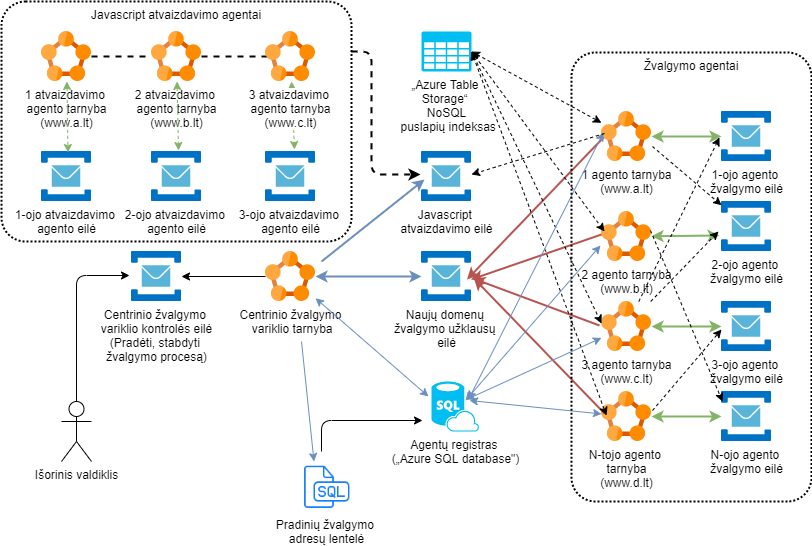
\includegraphics[scale=0.6]{img/Azure_Implementacija_Kasparo.png}
\caption{Struktūrinė prototipo sistemos schema}
\label{fig:azure_implementation_structural_scheme}
\end{figure}

\subsubsection{Duomenų saugojimo talpyklos}

Prototipas naudoja dvi talpyklas agentų informacijai ir puslapių peržiūros būsenai saugoti.

\subsubsubsection{Agentų registras}

„Azure SQL“ duomenų bazė, kurioje apibrėžta:

\begin{itemize}
    \item Peržiūros agentų registracijos lentelė
    \item Javascript atvaizdavimo agentų registracijos lentelė
    \item Pradinis peržiūros URL adresų sąrašas
    \item Javascript klientinio atvaizdavimo karkasų raktažodžių sąrašo lentelė, pagal kuriuos atliekama Javascript atvaizdavimo poreikio indentifikacija
\end{itemize}

 % Table generated by Excel2LaTeX from sheet 'crawling_vs_scraping'
\begin{table}[htbp]
  \centering
  \caption{Agentų registro lentelės schema \cite{MercedCloudBasedWebCrawler}}
    \begin{tabular}{|l|l|l|l|l|}
    \hline
    \textbf{Id} & \textbf{Agento\_Vardas} & \textbf{Agento\_Aptarnavimo\_Sritis} & \textbf{\textcolor{red}{Paskutinis\_Aktyvumas}} & \textbf{Ištrintas} \bigstrut\\
    \hline
    1 & A1 & abc.lt & 2020-05-02 15:30:15 & false \\
    \hline
    2 & A2 & def.lt & 2020-05-02 13:30:15 & true \\
    \hline
    \end{tabular}%
  \label{tab:agent_registry_table}%
\end{table}%
 
 \ref{tab:agent_registry_table} lentelėje pavaizduotame agentų registre raudonai pažymėtas paskutinio aktyvumo laiko stulpelis originaliai \cite{MercedCloudBasedWebCrawler} literatūroje neminėtas, tai -- rašto darbo autoriaus prototipo planavimo metu įgyvendinta korekcija siekiant atlaisvinti nebenaudojamus agentus.
 
 Įgyvendintas algoritmas, atlaisvinantis nebenaudojamus agentus, apibrėžiamas šiais žingsniais:
 
 \begin{enumerate}
     \item Gavus naujo domeno žvalgymo užklausą, centrinis žvalgymo variklis tikrina visų aktyvių agentų paskutinio aktyvumo stulpelio reikšmes
     \item Išrenkami visi agentai, kurių stulpelio „Paskutinis\_Aktyvumas“ reikšmė yra „NULL“ arba < DABARTINIS\_LAIKAS - NUSTATYMUOSE\_APIBRĖŽTAS\_NEAKTYVUMO\_PERIODAS 
     \item Kiekvienam išrinktam agentui tikrinama, ar jo peržiūros eilė yra tuščia, jei taip -- agentas naikinamas ir ištrinama jo peržiūros eilė
 \end{enumerate}
 
 \subsubsubsection{Puslapių indeksas}

Tai -- „Azure NoSQL Table Storage“ duomenų bazė, kurioje saugomi visi surasti URL adresai ir jų peržiūros būsena. \ref{tab:crawling_tablel} lentelėje nurodyta peržiūros URL adresų saugojimo lentelė. \textit{PartitionKey} apibrėžia domeno vardo sritį, o \textit{RowKey} -- MD5 kontroline suma užkoduotas pilnas URL adresas, kuris unikaliai identifikuoja puslapį jo domeno zonoje.

% Table generated by Excel2LaTeX from sheet 'Sheet1'
\noindent \hspace*{4em}%
\begin{table}[ht]
  \centering
  \caption{Peržiūros URL adresų lentelė}
    \begin{tabular}{|l|l|l|l|r|r|r|}
    \hline
    PartitionKey & RowKey & PageUrl & Timestamp & \multicolumn{1}{l|}{Visited} & \multicolumn{1}{l|}{StatusCode} & \multicolumn{1}{l|}{Rendered} \bigstrut\\
    \hline
    abc.lt & 0575118B9D... & abc.lt/naujienos/ & 2020-05-01T...& TRUE & 200 & TRUE \bigstrut\\
    \hline
    def.lt & 52F8F6432... & def.lt/orai & 2020-05-10T... & FALSE &     & FALSE \bigstrut\\
    \hline
    \end{tabular}%
  \label{tab:crawling_tablel}%
\end{table}%


\ref{tab:script_files_tablel} lentelėje pavaizduota skriptų saugojimo informacijos talpykla, kurioje saugomos HTML identifikuotų skriptų kontrolinės sumos ir Javascript atvaizdavimo sprendimas.

\pagebreak

\begin{itemize}
    \item \textit{PartitionKey} -- domeno vardo sritis
    \item \textit{RowKey} -- skripto URL adreso MD5 kontrolinė suma
    \item \textit{Checksum} -- skripto turinio MD5 kontrolinė suma
    \item \textit{ScriptFile} -- skripto pavadinimas
    \item \textit{RenderDecision} -- indikacija, ar rasta klientinio atvaizdavimo požymių
\end{itemize}

% Table generated by Excel2LaTeX from sheet 'Sheet1'
\begin{table}[ht]
  \centering
  \caption{Skriptų informacijos saugojimo lentelė}
    \begin{tabular}{|l|l|l|l|r|}
    \hline
    PartitionKey & RowKey & Checksum & ScriptFile & \multicolumn{1}{l|}{RenderDecision} \bigstrut\\
    \hline
    abc.lt & 0575118B9D... & 3d572837... & bundle.js & TRUE \bigstrut\\
    \hline
    def.lt & 52F8F64324... & 999101d8... & jquery.js & FALSE \bigstrut\\
    \hline
    \end{tabular}%
  \label{tab:script_files_tablel}%
\end{table}%


\subsubsection{Žvalgymo agentai}

Žvalgymo agentai įgyvendinti kaip „Service Fabric“ tarnybos be būsenos (angl. -- \textit{Stateless services}). Kiekvienas iš jų turi savo atitinkamą eilę, iš kurios ima žvalgytinų puslapių URL adresus. Priskirtoje „Service Bus“ eilėje talpinami tik tie puslapių URL adresai, kurie priklauso agentui priskirtai domeno vardo sričiai.

\subsubsection{Centrinis žvalgymo variklis}

Šis komponentas taip pat įgyvendintas, kaip „Service Fabric“ tarnyba be būsenos, jis sukuriamas iš karto paleidus klasterį ir yra atsakingas už naujų agentų ir jų žvalgymo eilių kūrimą/naikinimą. Šis komponentas klausosi 3 skirtingų „Service Bus“ eilių ir apdoroją jų žinutes:

\begin{itemize}
    \item \textbf{Centrinio žvalgymo variklio kontrolės eilė} -- į šią eilę roboto klientinė sąsaja talpina peržiūros komandas: pradėti, stabdyti peržiūros procesą, keisti aktyvių agentų skaičių
    \item \textbf{Naujų domenų žvalgymo užklausų eilė} -- tai pagrindinė „žvalgymo pasienio“ eilė, kurioje kaupiami visi URL adresai neturintys aktyvaus peržiūros agento. Jeigu agentas visgi egzistuoja, žvalgymo variklis atvykusį URL adresą peradresuoja jo atitinkamai žvalgymo eilei. Kitu atveju, žvalgymo variklis bando URL adresui kurti naują agentą, jei neviršytas maksimalus aktyvių agentų limitas
    \item \textbf{Javascript atvaizdavimo eilė} -- šioje eilėje talpinami URL adresai tų puslapių, kuriems buvo nustatyta indikacija, jog jie naudoja klientinį Javascript atvaizdavimo karkasą. Centrinis žvalgymo variklis gavęs žinutę iš šios eilės, patikrina, ar maksimalus aktyvių Javascript atvaizdavimo agentų skaičius neviršytas ir bando kurti atvaizdavimo agentą URL adreso domeno vardo sričiai.
\end{itemize}

\subsubsection{Javascript atvaizdavimo agentai}

Šių agentų veikimo principas beveik identiškas žvalgymo agentams -- jie turi savo domeno srities atvaizdavimo eiles. Skirtumas, jog pastarieji nenaudoja paprastų HTTP užklausų į URL adresu pasiekiamą žiniatinklio serverį, o pasitelkia kitoje „Service Fabric“ tarnyboje esančią „Chromium“ tvarkyklę, kuri turi integruotą Javascript atvaizdavimo variklį. Javascript atvaizdavimo agentai su šia tarnyba bendrauja per „Websocket“ protokolo jungtį, kuri leidžia tinklu kontroliuoti nutolusią naršyklę, tereikia paleidžiant tvarkyklę nurodyti parametrą, apibrėžiantį prisijungimo jungtį: \textit{chrome.exe --remote-debugging-port=9222}.

\subsection{Kiti prototipo realizacijoje panaudoti įrankiai}

Šiame poskyryje aprašomos įgyvendinant prototipą panaudotos bibliotekos, vykdomosios aplinkos, programavimo kalbos.

\subsubsection{Programavimo aplinka}

„Service Fabric“ klasterio kodas buvo rašytas C\# programavimo kalba panaudojant .NET Core 3.1 karkaso, kuris leidžia vienai kodo bazei veikti skirtingose operacinėse sistemose, versiją. Daug panaudotų „NuGet“ paketų valdymo sistemos bibliotekų (pvz.: PuppeteerSharp, AngleSharp) palaiko .NET Standard 2.0 versiją, kuri skirta tiek tradiciniam .NET karkasui, tiek ir .NET Core aplinkai.

\subsubsection{Bibliotekos}

\begin{itemize}
    \item \textit{AbotCrawler}\footnote{Abot -- https://github.com/sjdirect/abot} -- patogi ir aktyviai palaikoma .NET biblioteka, skirta specialiai puslapių žvalgymui. Įgyvendina daug žemo lygio funkcinių žvalgymo detalių (DNS išaiškinimas, žvalgymo intervalai, etiško žvalgymo politiką), todėl programuotojas gali papildomai nebesirūpinti jų įgyvendinimu
    \item \textit{Dapper} -- minimali ORM biblioteka, skirta komunikacijai su duomenų baze. Prototipui nereikėjo ORM bibliotekų, tokių kaip Entity Framework, funkcionalumo, todėl įgyvendinant achitektūrinį repozitorijos sluoksnį panaudotas šis paketas, kuris reikalauja rašyti užklausas rankomis \cite{DapperORM}
     \item \textit{AngleSharp} -- HTML dokumento apdorojimo .NET biblioteka, leidžianti serverio pusėje sukurti DOM medį, jį analizuoti, išgauti informaciją, keisti \cite{AngleSharp}. Panaudota Javascript skriptų išgavimui.
      \item \textit{PuppeteerSharp} -- komunikacijai su „Chromium“ tvarkykle naudojama .NET biblioteka, kuri originaliai sukurta Node.JS platformai \cite{PuppeteerSharp}. Ši biblioteka naudojama Javascript atvaizdavimo agentų prisijungimui „Websocket“ jungtimi prie „Chromium“ tvarkyklės agento
\end{itemize}

\subsection{Panaudojamumo atvejų dinamika}

Šiame poskyryje detaliau grafiškai pristatomos apibrėžtų panaudojamumo atvejų algoritminės sekos, kurios perteikiamos UML sekų diagramomis. 

\subsubsection{U1.1 Inicijuoti peržvalgos procesą}

Žemiau pateiktoje \ref{fig:initiate_crawling_uml_sequence} UML sekos diagramoje pavaizduotas sistemos administratoriaus inicijuojamas žvalgymo pradėjimo procesas, kurio metu pradinis URL adresų sąrašas perkeliamas į žvalgymo pasienio komponentą ir sukuriamas pradinis žvalgymo agentas.
\begin{figure}[ht!]
\centering
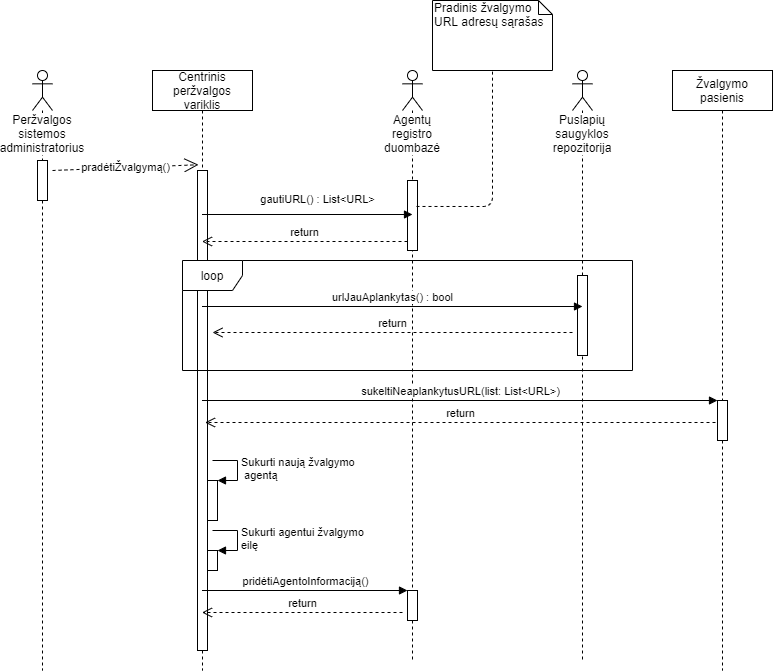
\includegraphics[scale=0.6]{img/initiate_crawling_process_sequence.png}
\caption{Žvalgymo inicijavimo proceso UML sekos diagrama}
\label{fig:initiate_crawling_uml_sequence}
\end{figure}

Peržvalgos sistemos administratorius yra klientinė programa, valdanti robotą. Galima realizuoti tiek žiniatinklio, tiek darbalaukinės programos klientą. Prototipo realizacijos metu klientas simuliuojamas naudojant „Service Bus Explorer“ eilių programą ir rankomis siunčiant žinutes į valdymo eilę.

\pagebreak

\subsubsection{U2 Vykdyti puslapio peržvalgą}

\ref{fig:perform_crawling_uml_sequence} UML sekos diagramoje pavaizduota žvalgymo agento darbo vykdymo schema. Akcentuotina, kad šis žvalgymo procesas kartojamas iki to laiko, kai žvalgymo agento eilė tampa tuščia ir po sistemos konfigūracijoje nustatyto agento neaktyvumo intervalo, Centrinis žvalgymo variklis tiesiog panaikina nebeaktyvų žvalgymo agentą.

\begin{figure}[ht!]
\hspace*{-2cm} 
\centering
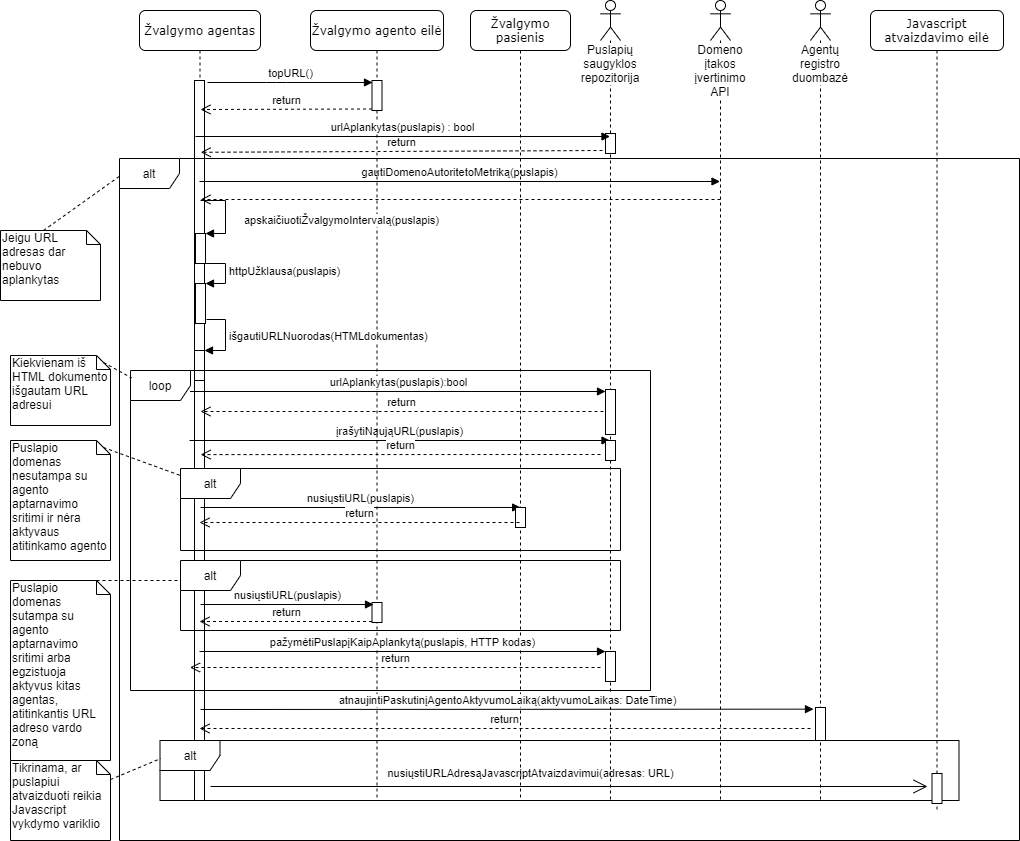
\includegraphics[scale=0.5]{img/perform_cralwing_sequence.png}
\caption{Žvalgymo vykdymo proceso UML sekos diagrama}
\label{fig:perform_crawling_uml_sequence}
\end{figure}

\subsubsection{U2.1 Įvertinti, ar puslapis vykdo klientinį Javascript atvaizdavimą}

\ref{fig:perform_crawling_uml_sequence} diagramoje paminėta, jog URL adresas po žvalgymo į Javascript atvaizdavimo eilę siunčiamas tik nustačius, jog puslapis reikalauja Javascript atvaizdavimo variklio, kad galėtų dinamiškai generuoti DOM medį. Šiame punkte pateikiama UML veiklos diagrama \ref{fig:js_rendering_condition}, kurioje nurodoma, kaip prototipinė sistema atlieka šį tikrinimą.

\begin{figure}[ht!]
\centering
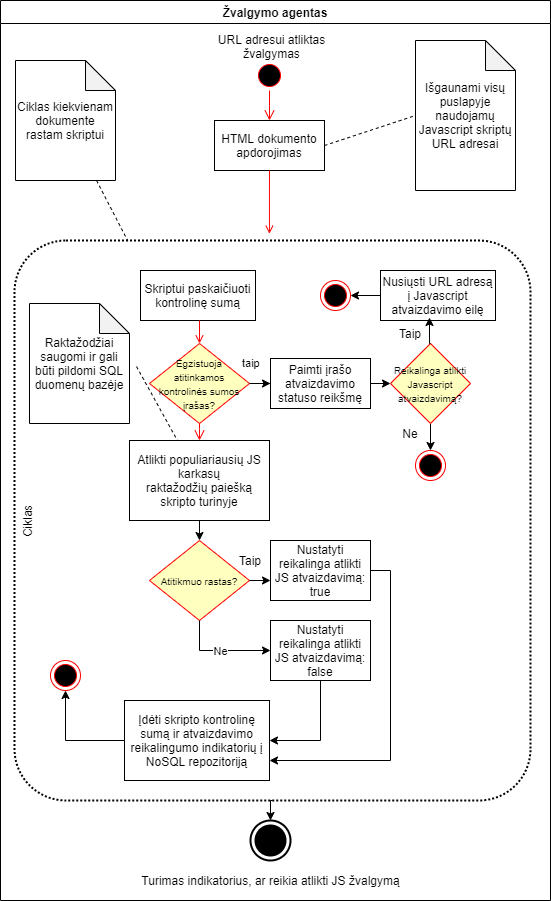
\includegraphics[scale=0.6]{img/javascript_rendering_condition_activity_diagram.png}
\caption{Poreikio atlikti Javascript atvaizdavimą indikatoriaus nustatymo UML veiklos diagrama}
\label{fig:js_rendering_condition}
\end{figure}

Šiame skyriuje aprašytos architektūros prototipo peržiūros greitaveika išbandoma eksperimentinio tyrimo, aprašyto 7 skyriuje, metu.